\documentclass{standalone}
\usepackage{ tikz }
\usepackage{ xparse }
\usepackage{../../../macros}
\usetikzlibrary{shapes}

\begin{document}
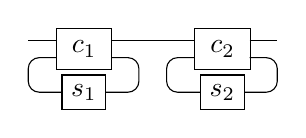
\begin{tikzpicture}[yscale=-1,x=1em,y=1.25em]
        
    \draw (0,0.5) -- (1,0.5);
    \node [draw, minimum height=1.5em, minimum width=2em, anchor=west] at (1,0.75) {$c_1$};
    \draw [rounded corners] (1,1) -- (0,1) -- (0,2) -- (1.2,2);
    \node [draw, minimum height=1em, minimum width=1.5em, anchor=west] at (1.2,2) {$s_1$};
    \draw [rounded corners] (2.8,2) -- (4,2) -- (4,1) -- (3,1);
 
    \draw (3, 0.5) -- (6, 0.5);
 
    \node [draw, minimum height=1.5em, minimum width=2em, anchor=west] at (6,0.75) {$c_2$};
    \draw [rounded corners] (6,1) -- (5,1) -- (5,2) -- (6.2,2);
    \node [draw, minimum height=1em, minimum width=1.5em, anchor=west] at (6.2,2) {$s_2$};
    \draw [rounded corners] (7.8,2) -- (9,2) -- (9,1) -- (8,1);
    \draw (8, 0.5) -- (9, 0.5);


\end{tikzpicture}
\end{document}